\section{Shared Memory}

In real shared memory there is no message-passing, node access one
shared memory. But in distributed system we simulate shared memory
using message passing.

\begin{itemize}
	\item A register represents each memory location (objects)
    \item Node can \texttt{read(R) => x}/\texttt{write(R, x)}
	\item Simplification of key-value stores
\end{itemize}

\paragraph{Basic Assumptions}
\begin{itemize}
    \item Nodes are sequential, they can only do one operation at a time.
invocation,response,invocation,response,\ldots
\item The values are positive integers initially zero.
    \end{itemize}

\paragraph{Definitions}
In an execution, an operation is
\begin{itemize}
	\item \textbf{complete} if both invocation \& response occured
	\item \textbf{failed} if invoked, but no response arrives
\end{itemize}

$op_1$ precedes $op_2$ if (denoted $<_p$) if response of $op_1$
precedes invocation of $op_2$. Otherwise they are concurrent.

\paragraph{Terminology}
\begin{itemize}
	\item (1,N)-algorithm: 1 designated writer, multiple readers
	\item (N,N)-algorithm: Multiple writers, multiple readers
\end{itemize}


\subsection{Regular Register (1,N)}
\begin{itemize}
	\item Termination: Each read and write operation of a correct node
	completes.
	\item Validity: Read return last value written if
		\begin{itemize}
			\item Read is not concurrent with another write, and
			\item Read is not concurrent with a failed operation
		\end{itemize}
	Otherwise the read must return the last value
	written or a concurrent value being written.
\end{itemize}


\subsubsection{Centralized Algorithm}

One process is designated as leader. For reading, the latest value must
be asked to the leader. For writing, leader's value is updated.

$\Rightarrow$ does not work if leader crashes.

\subsubsection{Bogus Algorithm}
\begin{itemize}
    \item[read]: return local value
    \item[write]: overwrite local value and broadcast change
\end{itemize}

\begin{figure}[!ht]
    \centering
        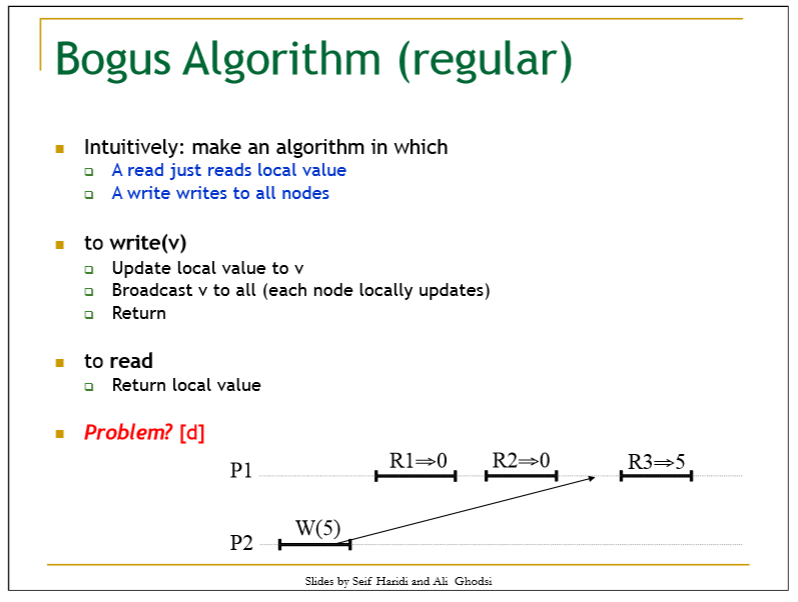
\includegraphics[width=6cm]{img/bogus_1.png}
        \caption{Bogus algorithm}
\end{figure}
\FloatBarrier{}

\paragraph{Read-one write all (1, N)}
Bogus algorithm modified can be use with a \textbf{perfect FD}
and fail-stop model.

\begin{itemize}
    \item[$\to$] write needs to wait \enquote{ACK} from all correct nodes when he
    broadcasts updated local value.
    \item[$\to$] read returns local value.
\end{itemize}

\subsubsection{Majority Voting Algorithm}
Main idea is based on a quorum principle,
\begin{itemize}
	\item Always write to and read from a majority of nodes
	\item At least one node knows most recent value
\end{itemize}

\paragraph{Quorum Principle}
Divide the system into quorums, any two quorums should intersect.
There are different type of quorum
\begin{itemize}
	\item Majority Quorum
		\begin{itemize}
            \item[Pro]: tolerate up to $\lceil N/2 \rceil -1$ crashes
            \item[Con]: Have to read/write $\lfloor N/2 \rfloor + 1$ values
		\end{itemize}
	\item Maekawa Quorum
		\begin{itemize}
			\item Arrange nodes in $M \times M$ grid ($M=sqrt(N)$)
			\item Write to rows, read to columns (always overlap)
            \item[Pro]: Only need to read/write $sqrt(N)$ nodes
            \item[Con]: Tolerate at most $sqrt(N)-1$ crashes
		\end{itemize}
\end{itemize}

\paragraph{Implementation}

\begin{table}[!ht]
    \begin{tabular}{>{\centering}m{0.2\linewidth}|m{0.7\linewidth}}
        \hline
        $read$ & \begin{enumerate}
                \item Broadcast read request
                    \begin{itemize}
                        \item[$\to$] receiver response with local value and seq\#
                    \end{itemize}
                \item Save values from majority of nodes
                \item Return value with highest seq\#
            \end{enumerate} \\
        \hline
        $write(v)$ & \begin{enumerate}
            \item Broadcast $v$ and seq\#
                \begin{itemize}
                    \item[$\to$] receiver update to $v$ \textcolor{red}{if newer seq\#}
                \end{itemize}
            \item Wait for ACK from majority of node then increments seq\#
        \end{enumerate} \\ \hline
    \end{tabular}
    \caption{Implementation of Majority Voting Algorithm (1,N)}
\end{table}
\FloatBarrier{}

The problem with the basic algorithm is that old write can overwrite
new write. (resolved by the added \textcolor{red}{red part})

\subsection{Single Storage}

\paragraph{Safety requirements}
\begin{itemize}
	\item \textbf{Sequential Consistency}: Only allow executions whose results
	appear as if there is a single system image and \enquote{local time} is
	obeyed
	\item \textbf{Linearizability/Atomicity}: Only allow executions whose
	results appear as if there is a single system image and
	\enquote{global time} is obeyed.
\end{itemize}

\paragraph{Liveness: progress\newline}

Liveness requirements: three progressively weaker versions
\begin{itemize}
	\item \textbf{Wait-free} (strongest): Every correct node should \enquote{make progress}
	(no deadkocks, no livelocks, no starvation)
	\item \textbf{Lock-free/non-blocking}: At least one correct node should
	\enquote{make progress} (no deadlocks, no livelock, maybe starvation)
	\item \textbf{Obstruction free/solo-termination}: If a single node executes
	without interference (contention) it makes progress
	(no deadlocks, maybe livelocks, maybe starvation)
\end{itemize}

\subsection{Atomic/Linearizable Registers}

\begin{itemize}
	\item Termination (Wait-freedom): If a node is correct, each read and write op
	eventually completes
	\item Linearization Points:
	\begin{itemize}
		\item \textbf{Read ops} appears as if immediately happened at all nodes
		at some time between invocation and response.
		\item \textbf{Write ops} appears as if immediately happened at all nodes
		at some time between invocation and response.
		\item \textbf{Failed ops} appears as whether completed at every node
		whether never occured at any node
	\end{itemize}

    \paragraph{Equivalent with}
    \begin{itemize}
        \item Validity: read
            \begin{enumerate}
                \item[IF] read not conurrent with another write or with a failed operation
                    return last value written
                \item[ELSE] return concurrent value written
            \end{enumerate}
        \item Ordering: if read $r_1$ precede read $r_2$ then write $r1$ precedes $r2$
    \end{itemize}
\end{itemize}

\paragraph{Majority voting}
There is a problem with the majority voting as the system could appear
as non atomic.

\subsubsection{Atomic register: Single writer (1,N))}

Solution to previous issues: when reading, also make a write before responding.

$\Rightarrow$ Use \textbf{causality} to enforce \textbf{atomicity}.

\begin{figure}[!ht]
    \centering
    \begin{tabular}{m{7cm}m{7cm}}
		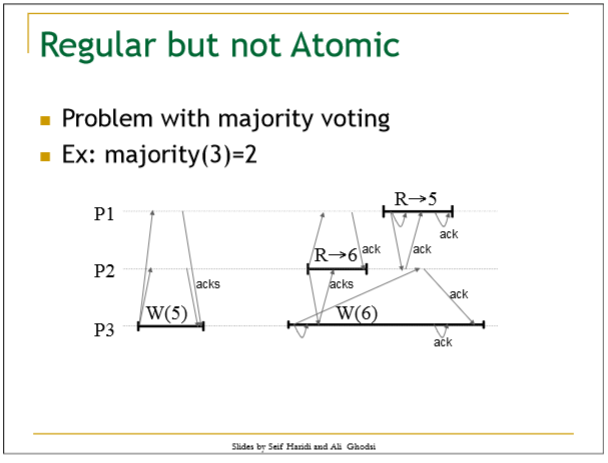
\includegraphics[width=7cm]{img/maj_prob.png}&
		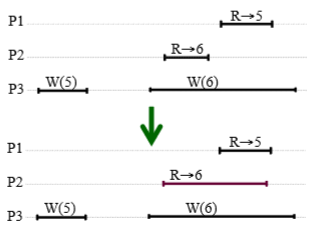
\includegraphics[width=6cm]{img/maj_sol.png}
	\end{tabular}
		\caption{Majority Voting Problem and Solution}
\end{figure}
\FloatBarrier{}

\subsubsection{Atomic register: Multiple writers (N,N))}

With multiple writers, their seq\# might be non-synchronized
which has the effect of ignoring some write operations.

\paragraph{Solution}
\begin{enumerate}
	\item Get seq\# before writing by reading from
	the majority (to get last seq\#)
	\item Send Ack if receive write with old \#seq
\end{enumerate}

\paragraph{Message passing}
Message passing can be simulated using shared memory. The idea
consist of using a register AB to simulate the channel between A and B like a pipe.

\begin{itemize}
    \item $\to$ Message passing and shared memory equivalent in functionality
but not in always in efficiency.
\end{itemize}

\subsection{Linearizability}
\subsubsection{Formalism}
\begin{itemize}
	\item $R-inv_i(X)$ Read invocation by node i on register X
	\item $R-res_i(a)$ Response with value a to read by node i
	\item $W-inv_i(X,a)$ Write invocation by node i on register
	X with value a.
	\item $W-res_i$ Response (confirmation) to write by node i
\end{itemize}

\subsubsection{Executions}
Every execution consists of:
\begin{itemize}
	\item Read operations composed of two events:
	$R-inv_i(X)$ and $R-res_i(a)$
	\item Write operations which consist of two events:
	$W-inv_i(X,a)$ and $W-res_i$
	\item An execution is sequential if:
	\begin{itemize}
		\item X-inv by $i$ immediately followed by a corresponding X-res at $i$
		\item X-res by $i$ immediately follows a corresponding X-inv by $i$
		\item no concurrency, read $x$ by $p_1$, write $y$ by $p_5$,\ldots
	\end{itemize}
\end{itemize}

\subsubsection{Assumptions}
\begin{itemize}
    \item An operation $O$ is \textbf{pending} in execution $E$ if $O$ has no
    response event
    \item An execution is \textbf{complete} if every operation is complete
    (else partial)
    \item An operation $X$ \textbf{precedes} operation $Y$ in execution $E$ if
    response of $X$ is before invocation of $Y$ in $E$
    \end{itemize}

\subsubsection{Linearizability formally}

Consider two executions $E$ and $F$.

\begin{table}[!ht]
    \begin{tabular}{p{0.475\linewidth}|p{0.475\linewidth}}
        Linearizability w/o failure (sequential consistency) & Linearizability with failure (partial execution) \\
        \hline
        A complete $E$ is \textbf{linearizable} if $\exists$ F s.t.
        \begin{itemize}
            \item \textbf{Similarity} events(E) = events(F)
            \item \textbf{No concurrency} F is sequential
            \item \textbf{Legal operations}
            \item \textbf{Time ordering} if $X \preceq Y$ in $E$, $X \preceq Y$ in $F$
        \end{itemize} & A partial $E$ is \textbf{linearizable} if $E$ is modified s.t.
        \begin{itemize}
            \item Every pending operation is completed by
            \begin{itemize}
                \item removing the invocation of the operation, or
                \item adding a response to the operation
            \end{itemize}
            \item $F$ is linearizable
        \end{itemize} \\
    \end{tabular}
\end{table}
\FloatBarrier{}
